\documentclass[aip,jcp,reprint,noshowkeys,superscriptaddress]{revtex4-1}
\usepackage{graphicx,dcolumn,bm,xcolor,microtype,multirow,amscd,amsmath,amssymb,amsfonts,physics,wrapfig,txfonts,siunitx}
\usepackage[version=4]{mhchem}
%\usepackage{natbib}
\bibliographystyle{achemso}

\newcommand{\ie}{\textit{i.e.}}
\newcommand{\eg}{\textit{e.g.}}
\newcommand{\alert}[1]{\textcolor{black}{#1}}
\usepackage[normalem]{ulem}
\newcommand{\fk}[1]{\textcolor{blue}{#1}}
\newcommand{\titou}[1]{\textcolor{red}{#1}}
\newcommand{\trashPFL}[1]{\textcolor{red}{\sout{#1}}}
\newcommand{\PFL}[1]{\titou{(\underline{\bf PFL}: #1)}}
\newcommand{\toto}[1]{\textcolor{green}{#1}}
\newcommand{\trashAS}[1]{\textcolor{green}{\sout{#1}}}
\newcommand{\AS}[1]{\toto{(\underline{\bf AS}: #1)}}
\newcommand{\ant}[1]{\textcolor{orange}{#1}}
\newcommand{\SupInf}{\textcolor{blue}{Supporting Information}}

\newcommand{\mc}{\multicolumn}
\newcommand{\fnm}{\footnotemark}
\newcommand{\fnt}{\footnotetext}
\newcommand{\tabc}[1]{\multicolumn{1}{c}{#1}}
\newcommand{\QP}{\textsc{quantum package}}

\newcommand{\EHF}{E_\text{HF}}
\newcommand{\EDOCI}{E_\text{DOCI}}
\newcommand{\EFCI}{E_\text{FCI}}
\newcommand{\Ndet}{N_\text{det}}
\newcommand{\Nbas}{N}

\usepackage[
	colorlinks=true,
    citecolor=blue,
    breaklinks=true
	]{hyperref}
\urlstyle{same}

\begin{document}

\newcommand{\LCPQ}{Laboratoire de Chimie et Physique Quantiques (UMR 5626), Universit\'e de Toulouse, CNRS, UPS, France}

\title{Title}

\author{F\'abris Kossoski}
\email{fkossoski@irsamc.ups-tlse.fr}
\affiliation{\LCPQ}
\author{Pierre-Fran\c{c}ois Loos}
\email{loos@irsamc.ups-tlse.fr}
\affiliation{\LCPQ}

% Abstract
\begin{abstract}
{\bf Abstract:} 
\bigskip
\begin{center}
        \boxed{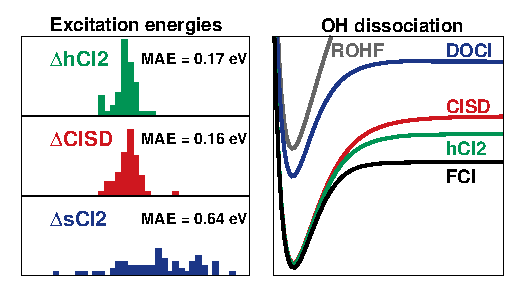
\includegraphics[keepaspectratio,width=2in]{TOC}}
\end{center}
\bigskip
\end{abstract}

% Title
\maketitle


%%%%%%%%%%%%%%%%%%%%%%%%%%%%%%%%%%%%%%%%%%%%%%%%%%
%\section{Introduction}
%\label{sec:intro}
%%%%%%%%%%%%%%%%%%%%%%%%%%%%%%%%%%%%%%%%%%%%%%%%%%

%%%%%%%%%%%%%%%%%%%%%%%%%%%%%%%%%
%\section{Computational details}
%\label{sec:compdet}
%%%%%%%%%%%%%%%%%%%%%%%%%%%%%%%%

%%%%%%%%%%%%%%%%%%%%%%%%%%%%%%%%
%\section{Results and discussion}
%\label{sec:res}
%%%%%%%%%%%%%%%%%%%%%%%%%%%%%%%%

%%%%%%%%%%%%%%%%%%%%%%%%%%%%%%%%
%\section{Conclusion and perspectives}
%\label{sec:ccl}
%%%%%%%%%%%%%%%%%%%%%%%%%%%%%%%%

%%%%%%%%%%%%%%%%%%%%%%%%%%%%%%%%
\begin{acknowledgements}
This work was performed using HPC resources from CALMIP (Toulouse) under allocation 2021-18005.
This project has received funding from the European Research Council (ERC) under the European Union's Horizon 2020 research and innovation programme (Grant agreement No.~863481).
\end{acknowledgements}
%%%%%%%%%%%%%%%%%%%%%%%%%%%%%%%%

%%%%%%%%%%%%%%%%%%%%%%%%%%%%%%%%%%
\section*{Supporting information available}
\label{sec:SI}
%%%%%%%%%%%%%%%%%%%%%%%%%%%%%%%%%%

%%%%%%%%%%%%%%%%%%%%%%%%%%%%%%%%
%\section*{Data availability statement}
%%%%%%%%%%%%%%%%%%%%%%%%%%%%%%%%
%The data that support the findings of this study are openly available in Zenodo at \href{http://doi.org/XX.XXXX/zenodo.XXXXXXX}{http://doi.org/XX.XXXX/zenodo.XXXXXXX}.

%%%%%%%%%%%%%%%%%%%%%%%%%%%%%%%%
\bibliography{manuscript}
%%%%%%%%%%%%%%%%%%%%%%%%%%%%%%%%

\end{document}
